%----------------------------------------------------------------
%
%  File    :  survey-style.tex
%
%  Author  :  Dominik Mocher, not  IICM, TU Graz, Austria
% 
%  Created :  27 May 93
% 
%  Changed :  19 Feb 2004
% 
%----------------------------------------------------------------


\chapter{Cell Visualization Techniques}\label{chap:celltypes}


\section{What to Visualize in Cells?}
Often graph node links contain additional data, besides their connected nodes and weight, for example the textual description.

Most of the time, the cell simply represents the connection between two nodes by filling the cell. If the input is a weighted graph, this information is often extended by the edge weights. Given the case that the input graph is undirected, the matrix forms a symmetric pattern along the diagonal. 

On the other hand, the cell can also represent data of a node, for example the affiliation to a specific cluster or the similarity to nodes from other clusters or the local neighborhood. 
Most tools provide the possibility to highlight the current selection in the matrix.

\section{How to visualize it in cells?}

Connections are most of the time shown in a black-white scheme, where black means that there is a connection, and accordingly white shows, that there is none. The current selection is then highlighted by increasing the transparency of the not-selected cells or simply setting them to grey. The logical next step from this is the extension to a wider color scheme, so that for example weights can be represented by different color grades, additionally with text as a fallback. If this scale is discrete, there is also the possibility to display icons or textures instead of color grades.
If the data which should be visualized is more exotic, like the similarity of nodes in the local neighborhood, this could be displayed as bar charts or histograms inside the cells. A matrix cell can even include another matrix and represent the according sub-cells. This technique is mainly used to simplify complex and large matrices.


\section{Example: Nodetrix}


\begin{figure}[H]
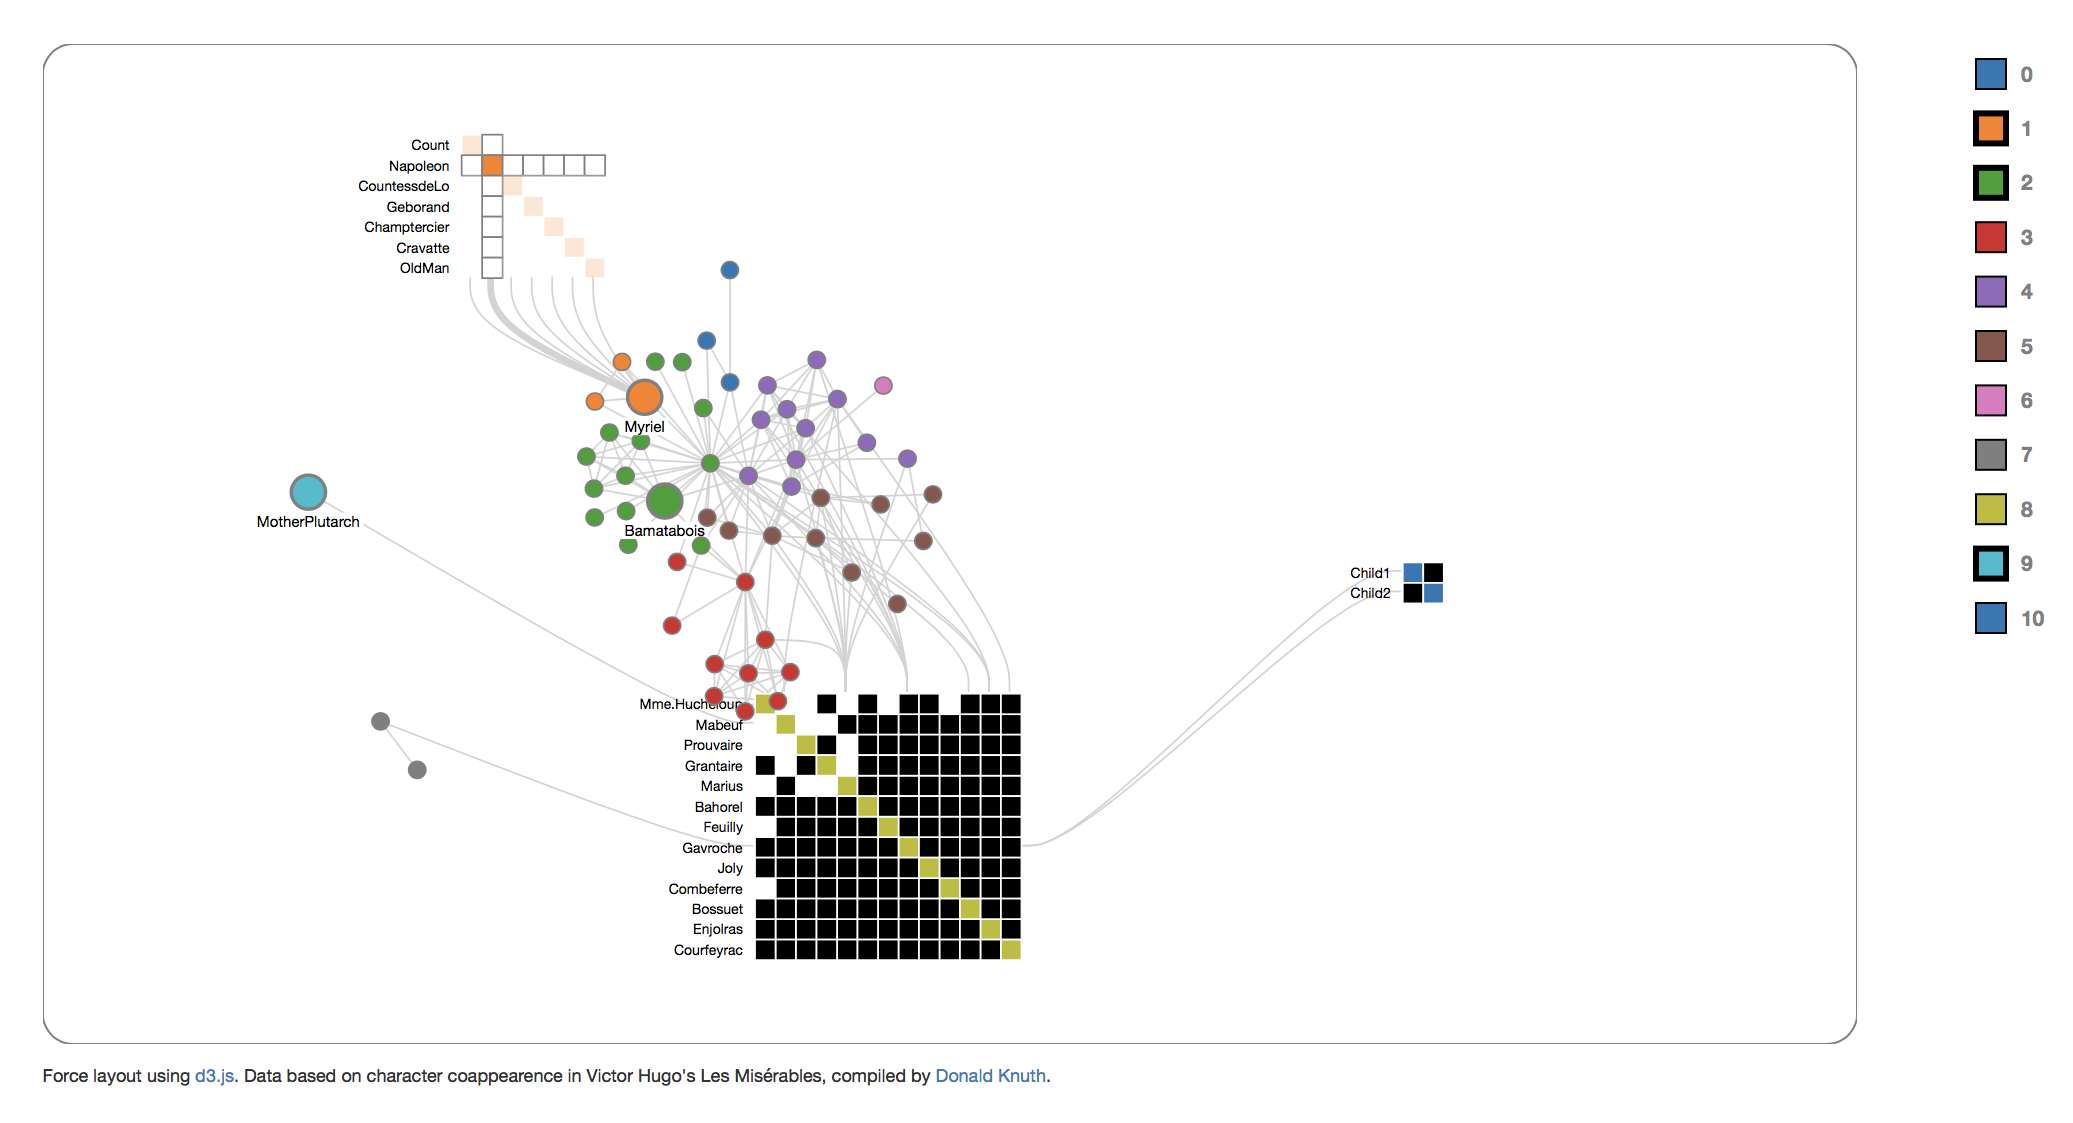
\includegraphics[width=\textwidth]{images/nodetrix_cell}
\caption{The demo application of Nodetrix. Screenshot created using Nodetrix. \citep[1302-1309]{henry-nodetrix-2007}.\label{fig:cell_nodetrix}}
\end{figure}



In the matrix representation of Nodetrix in figure \ref{fig:cell_nodetrix} can be seen, that connections are shown as black cells and the color in the matrix diagonal visualizes the affiliation to a specific cluster in the graph. The matrices in Nodetrix have a hover effect, which highlights the row and column of the currently selected cell. Every other cell in the matrix becomes light gray to help the user focus on connections. Additionally, the connections to graph nodes from the selected cell are emphasized too, as they are drawn boldly. \citep[1302-1309]{henry-nodetrix-2007}

\section{Example: Matrix Zoom}

\begin{figure}[H]
\centering
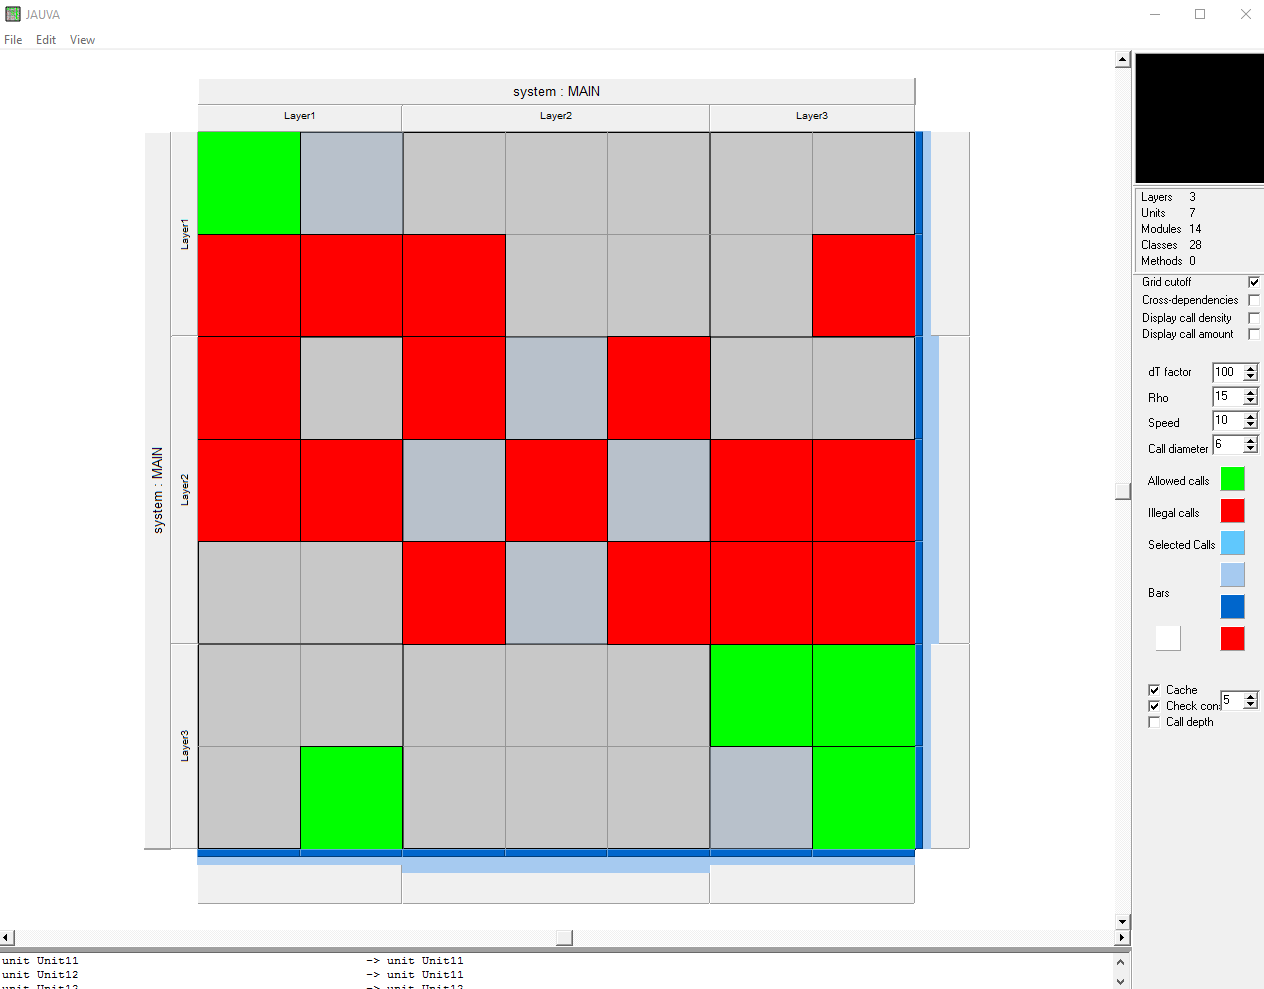
\includegraphics[width=0.8\textwidth]{images/matrixzoom_cell}
\caption{The color encoding of Matrix Zoom. Screenshot created using Matrix Zoom. \citep[227--232]{ham-ivis-2003}\label{fig:zell_matrixzoom}}
\end{figure}

Matrix zoom uses colors to visualize edge attributes, as shown in figure \ref{fig:zell_matrixzoom}. In the example set, edge attributes are an indication if a call is allowed or not or the local neighborhood of a call, visualized in a color scale. Therefore, calls, which have a shorter path-distance to the considered call are indicated in red. Transparency is used to indicate the call density of this matrix cell, higher cell density meaning a larger percentage of sub cells containing calls. \citep[227--232]{ham-ivis-2003}


\section{Example: Cubix}

\begin{figure}[H]
\centering
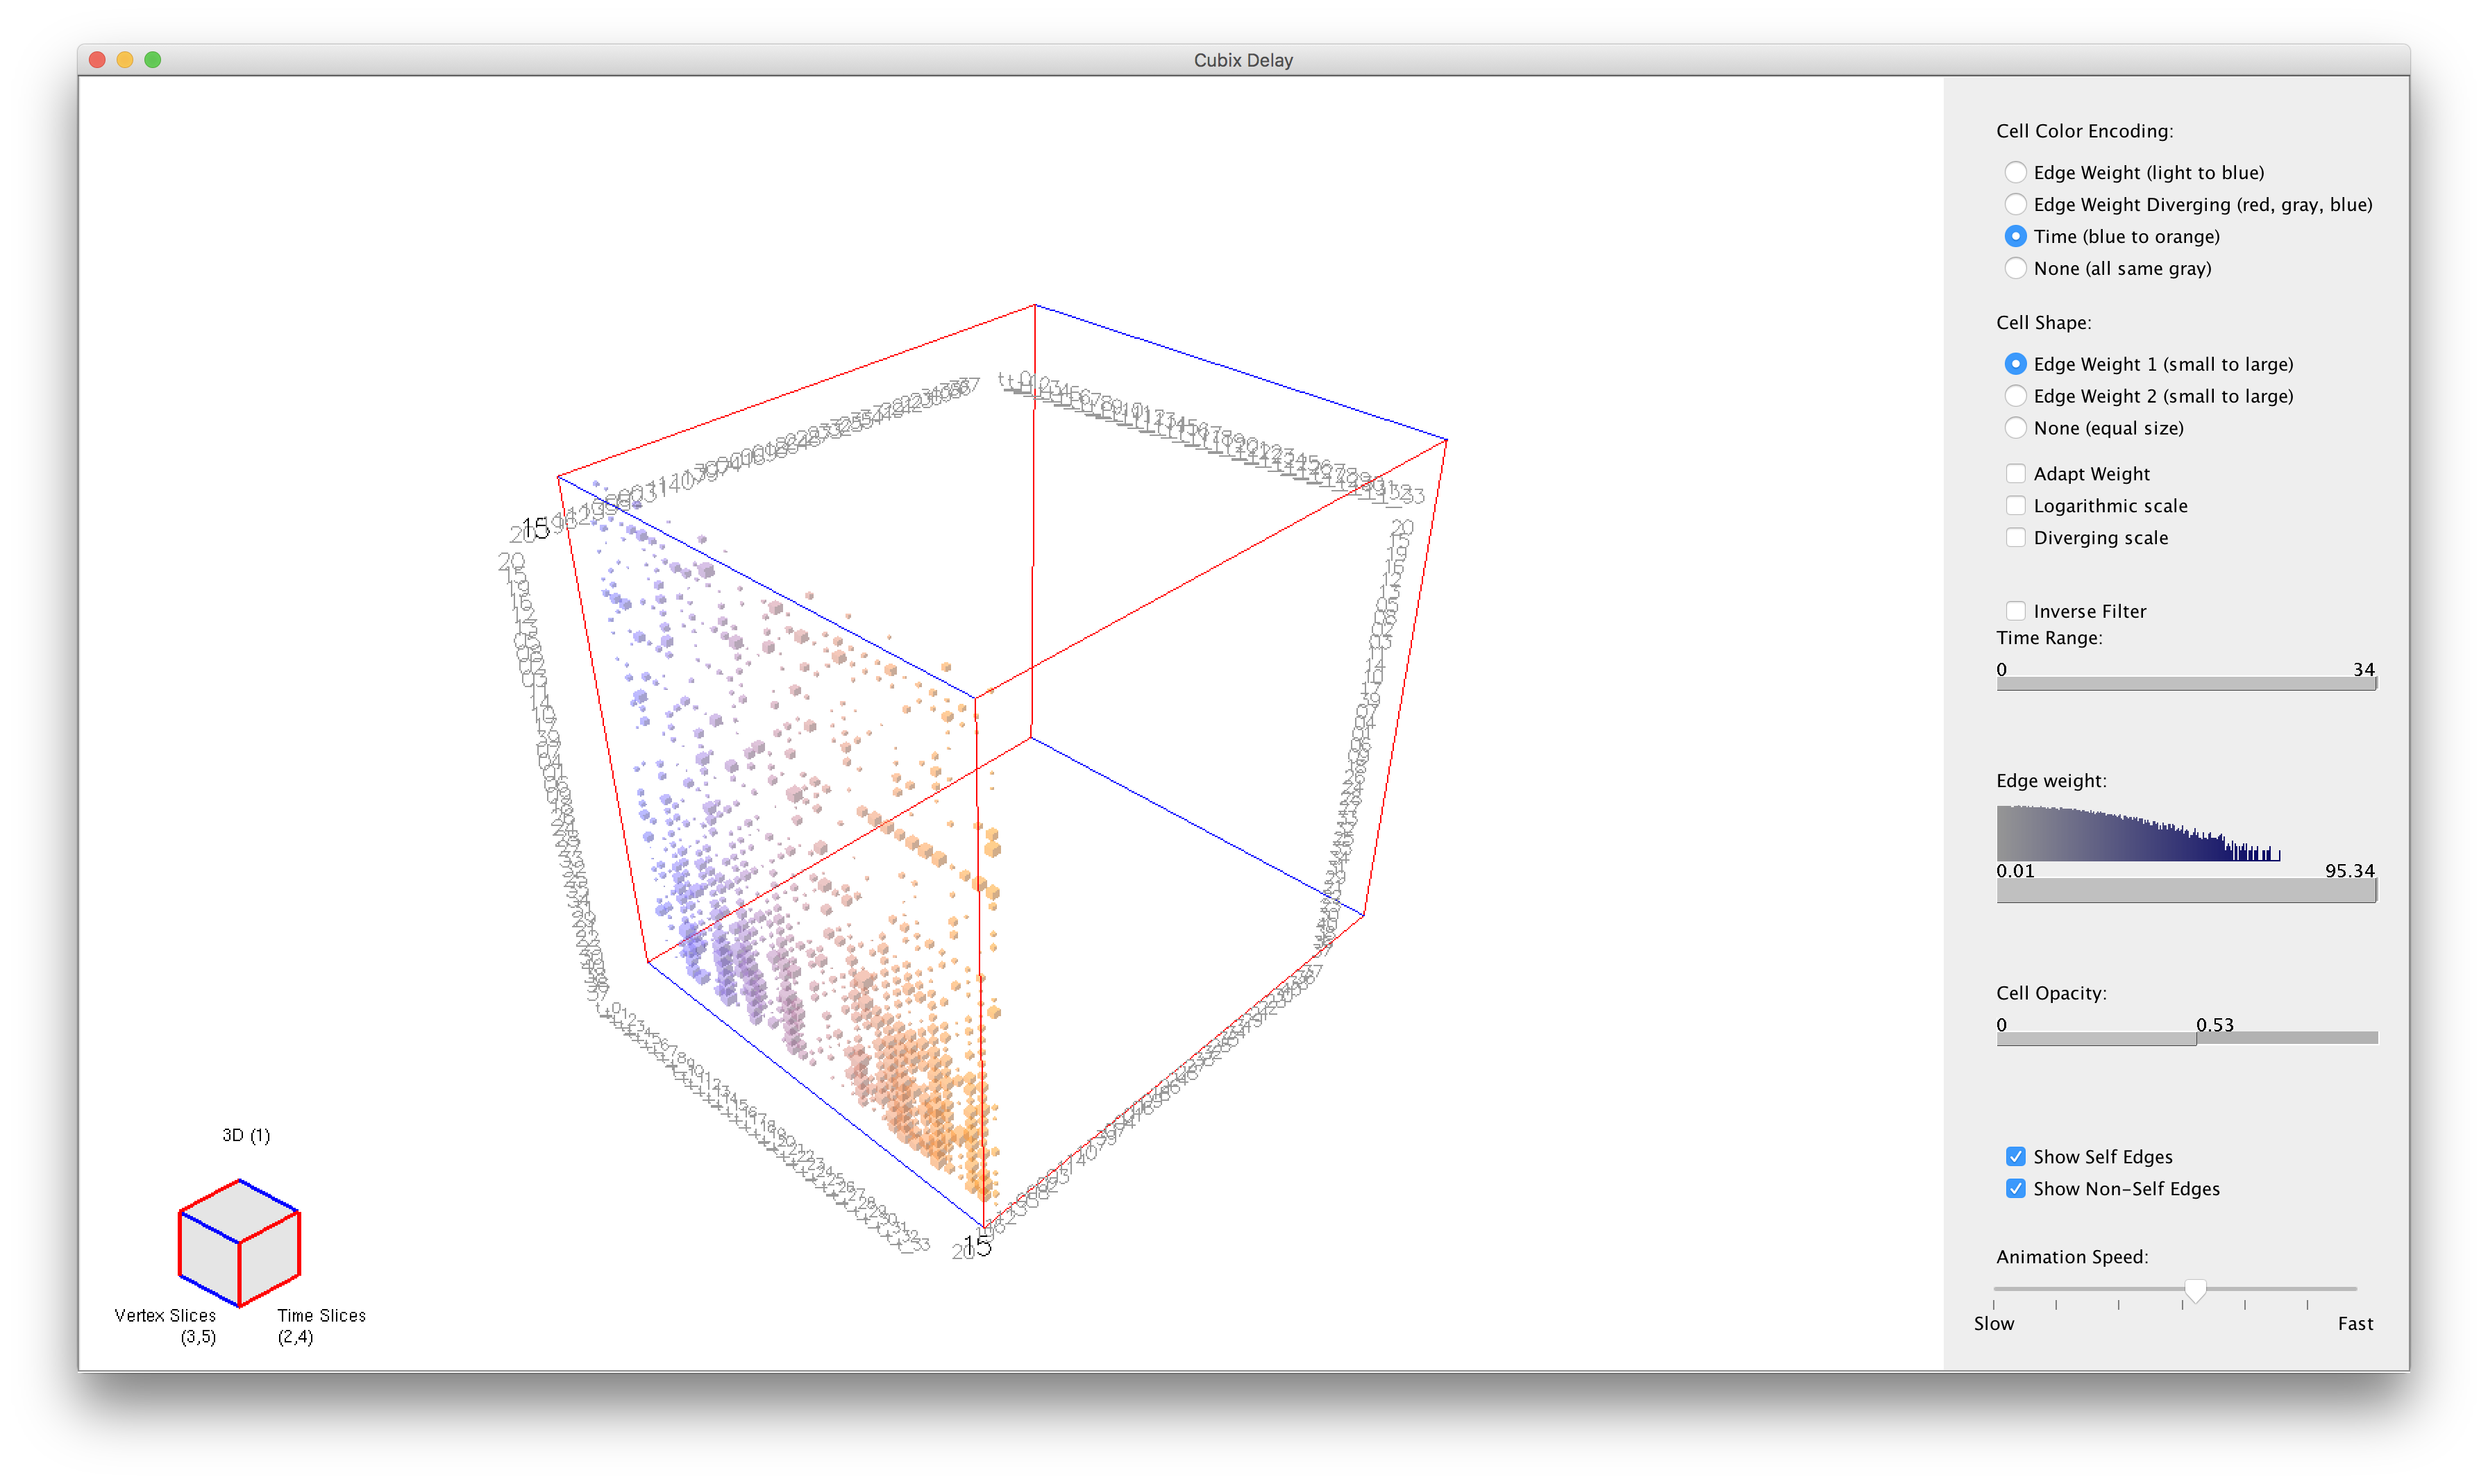
\includegraphics[width=0.8\textwidth]{images/cubix3d_cell}
\caption{The 3D representation of Data in Cubix, screenshot created using Cubix.\citep[877--886]{bach-cubix-2014}\label{fig:cell_cubix3d}}
\end{figure}

\begin{figure}[H]
\centering
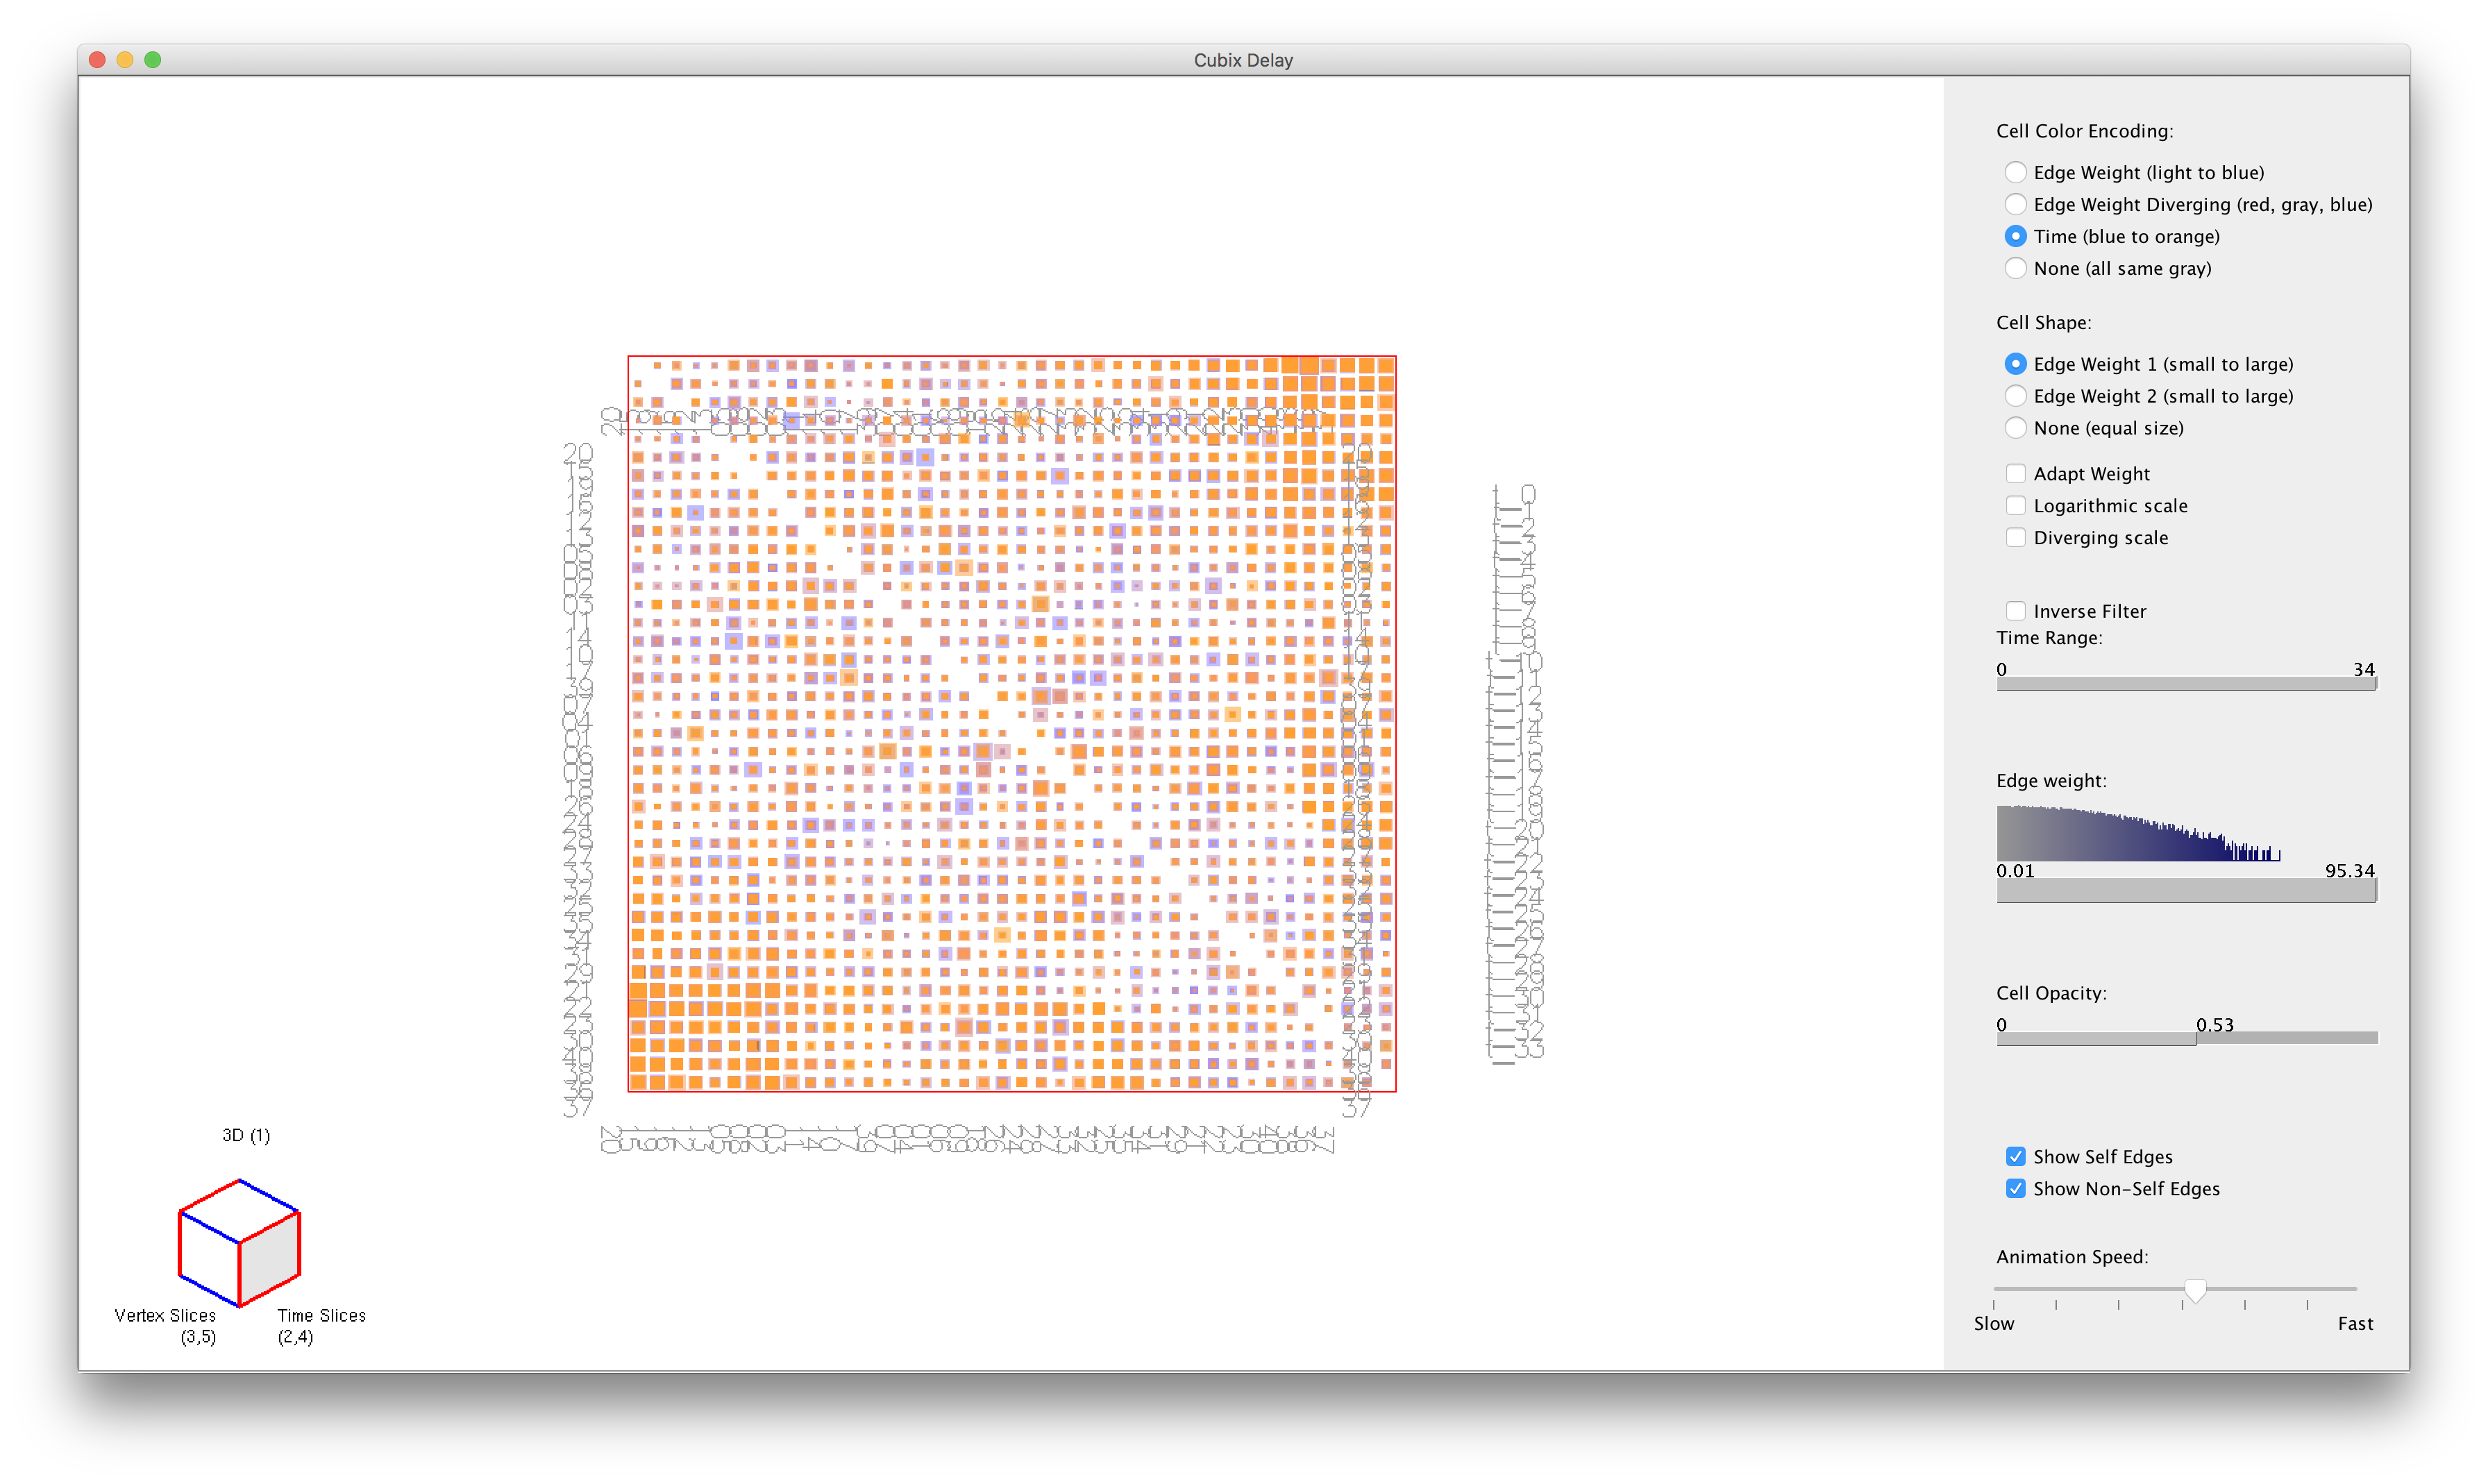
\includegraphics[width=0.8\textwidth]{images/cubix2d_cell}
\caption{The same data in 2D shown as time slices, screenshot created using Cubix. \citep[877--886]{bach-cubix-2014}\label{fig:cell_cubix2d}}
\end{figure}


Cubix is a tool to visualize and analyze graphs, which changes over time using the space-time-metaphor. Adjacency matrices are stacked onto each other in chronological order to create a cube with two vertex and one time dimension, as it is shown in figure \ref{fig:cell_cubix3d}.

The cell colors represent by default the edge weight, this can also be changed to the edge weight diverging or the affiliation to a specific time slice. The user can switch off the color encoding too, for easier recognizing patterns of the cells. Since this is a three-dimensional visualization, cell opacity is an important method for identifying patterns or cells behind another one. For further investigation, a single time slice can be inspected as seen in figure \ref{fig:cell_cubix2d}

Additionally, the size of the cell is another tool to visualize the weight of the edges and their change over time. For pattern finding, this feature can also be turned off.  \citep[877--886]{bach-cubix-2014}
